%%%%%%%%%%%%%%%%%%%%%%%%%%%%%%%%%%%%%%%%%%%%
% En 'inclues.tex' se encuentran la importación de paquetes necesarios
%%%%%%%%%%%%%%%%%%%%%%%%%%%%%%%%%%%%%%%%%%%%
%%%%%%%%%%%%%%%%%%%%%%%%%%%%%%%%%%%%%%%%%
% University Assignment Title Page 
% LaTeX Template
% Version 1.0 (27/12/12)
%
% This template has been downloaded from:
% http://www.LaTeXTemplates.com
%
% Original author:
% WikiBooks (http://en.wikibooks.org/wiki/LaTeX/Title_Creation)
%
% License:
% CC BY-NC-SA 3.0 (http://creativecommons.org/licenses/by-nc-sa/3.0/)
% 
% Instructions for using this template:
% This title page is capable of being compiled as is. This is not useful for 
% including it in another document. To do this, you have two options: 
%
% 1) Copy/paste everything between \begin{document} and \end{document} 
% starting at \begin{titlepage} and paste this into another LaTeX file where you 
% want your title page.
% OR
% 2) Remove everything outside the \begin{titlepage} and \end{titlepage} and 
% move this file to the same directory as the LaTeX file you wish to add it to. 
% Then add \input{./title_page_1.tex} to your LaTeX file where you want your
% title page.
%
%%%%%%%%%%%%%%%%%%%%%%%%%%%%%%%%%%%%%%%%%
%\title{Title page with logo}
%----------------------------------------------------------------------------------------
%	PACKAGES AND OTHER DOCUMENT CONFIGURATIONS
%----------------------------------------------------------------------------------------
\documentclass[14pt]{extarticle}
%Paquetes para idioma español y codifcación UTF8
\usepackage[spanish]{babel}
\usepackage[utf8x]{inputenc}
%natbib, para bibliografía y referencias
\usepackage[numbers]{natbib}
%paquete de matemática, vuela
\usepackage{amsmath}
%fuente 'fourier'
\usepackage{fourier}
%paquete para URLs
\usepackage{url}
%paquete para ubicar las imágenes
\usepackage{float}
%paquete para imágenes y en dónde las tiene que buscar
\usepackage{graphicx}
\graphicspath{{images/}}
%paquete para epígrafes
\usepackage{subcaption}
%paquete para definir los márgenes de la hoja
\usepackage[left=2cm,right=2cm,top=4cm,bottom=4cm]{geometry}
%paquete para poner todos y comentarios
\usepackage[colorinlistoftodos]{todonotes}
%paquete para trabajar con código
\usepackage{listings}
%paquete para trabajar con colores y definir propios
\usepackage{color}

%Cabeceras
\usepackage{fancyhdr}
\pagestyle{fancy}
\fancyhead[L]{Bases de Datos II, 2018}
\fancyhead[C]{}
\fancyhead[R]{UNPSJB}

\fancyfoot[R]{Luciano Serruya Aloisi}
\fancyfoot[L]{Trabajo Práctico 2}

%%paquete para reducir espacio entre secciones
%\usepackage{titlesec}
%\titlespacing*{\section}{0pt}{1.1\baselineskip}{\baselineskip}

%Comando para poner doble comillas más fácil
\newcommand{\dq}[1]{``#1''}

\definecolor{mygreen}{rgb}{0,0.6,0}
\definecolor{mygray}{rgb}{0.5,0.5,0.5}
\definecolor{mymauve}{rgb}{0.58,0,0.82}
\definecolor{dkgreen}{rgb}{0,0.6,0}
\definecolor{ltgray}{rgb}{0.5,0.5,0.5}
\definecolor{alizarin}{rgb}{0.82, 0.1, 0.26}

\lstdefinestyle{customstyle}{ 
  backgroundcolor=\color{white},   % choose the background color; you must add \usepackage{color} or \usepackage{xcolor}; should come as last argument
  basicstyle=\footnotesize,        % the size of the fonts that are used for the code
  breakatwhitespace=false,         % sets if automatic breaks should only happen at whitespace
  breaklines=true,                 % sets automatic line breaking
  captionpos=b,                    % sets the caption-position to bottom
  commentstyle=\color{mygreen},    % comment style
  escapeinside={\%*}{*)},          % if you want to add LaTeX within your code
  extendedchars=true,              % lets you use non-ASCII characters; for 8-bits encodings only, does not work with UTF-8
  frame=single,	                   % adds a frame around the code
  keepspaces=true,                 % keeps spaces in text, useful for keeping indentation of code (possibly needs columns=flexible)
  keywordstyle=\color{blue},       % keyword style
  language=Octave,                 % the language of the code
  numbers=left,                    % where to put the line-numbers; possible values are (none, left, right)
  numbersep=5pt,                   % how far the line-numbers are from the code
  numberstyle=\tiny\color{mygray}, % the style that is used for the line-numbers
  rulecolor=\color{black},         % if not set, the frame-color may be changed on line-breaks within not-black text (e.g. comments (green here))
  showspaces=false,                % show spaces everywhere adding particular underscores; it overrides 'showstringspaces'
  showstringspaces=false,          % underline spaces within strings only
  showtabs=false,                  % show tabs within strings adding particular underscores
  stepnumber=2,                    % the step between two line-numbers. If it's 1, each line will be numbered
  stringstyle=\color{mymauve},     % string literal style
  tabsize=2,	                   % sets default tabsize to 2 spaces
  title=\lstname                   % show the filename of files included with \lstinputlisting; also try caption instead of title
}

\lstdefinestyle{sql}{
	basicstyle=\fontsize{12}{10}\ttfamily,
	belowcaptionskip=1\baselineskip,
  	breaklines=true,
  	title=\lstname,	% show the filename of files included with \lstinputlisting; also try caption instead of title
  	frame=L, %Este pone la línea (doble) separadora a la izquiera, ir probando entre l, L,r y R
  	xleftmargin=\parindent,
  	language=SQL,
  	morekeywords={*,modify,MODIFY,...},
  	numbers=left,                    % where to put the line-numbers; possible values are (none, left, right)
  	numberstyle=\color{mygray}, % the style that is used for the line-numbers
  	rulecolor=\color{mygray},         % if not set, the frame-color may be changed on line-breaks within not-black text (e.g. comments (green here))
  	showstringspaces=false,
  	captionpos=b,                    % sets the caption-position to bottom
  	keywordstyle=\bfseries\color{green!40!black},
  	commentstyle=\itshape\color{purple!40!black},
  	identifierstyle=\color{blue},
  	stringstyle=\color{alizarin},
  	escapechar=@,
}

\lstdefinestyle{cli}{
    basicstyle=\fontsize{12}{10}\ttfamily,%\fontfamily{phv}\selectfont,
	belowcaptionskip=1\baselineskip,
  	breaklines=true,
  	title=\lstname,	% show the filename of files included with \lstinputlisting; also try caption instead of title
  	%frame=L, %Este pone la línea (doble) separadora a la izquiera, ir probando entre l, L,r y R
  	xleftmargin=\parindent,
  	language=bash,
  	%numbers=left,                    % where to put the line-numbers; possible values are (none, left, right)
  	%numberstyle=\color{mygray}, % the style that is used for the line-numbers
  	%rulecolor=\color{mygray},         % if not set, the frame-color may be changed on line-breaks within not-black text (e.g. comments (green here))
  	showstringspaces=false,
  	captionpos=b,                    % sets the caption-position to bottom
  	keywordstyle=\bfseries\color{blue!40!black},
  	commentstyle=\itshape\color{purple!40!black},
  	identifierstyle=\color{blue},
  	stringstyle=\color{alizarin},
  	escapechar=@,
}

\lstdefinestyle{bash}{
	basicstyle=\fontsize{12}{10}\ttfamily,
	belowcaptionskip=1\baselineskip,
  	breaklines=true,
  	%title=\lstname,	% show the filename of files included with \lstinputlisting; also try caption instead of title
  	%frame=L, %Este pone la línea (doble) separadora a la izquiera, ir probando entre l, L,r y R
  	xleftmargin=\parindent,
  	language=bash,
  	%numbers=left,                    % where to put the line-numbers; possible values are (none, left, right)
  	numberstyle=\color{mygray}, % the style that is used for the line-numbers
  	rulecolor=\color{mygray},         % if not set, the frame-color may be changed on line-breaks within not-black text (e.g. comments (green here))
  	showstringspaces=false,
  	captionpos=b,                    % sets the caption-position to bottom
  	keywordstyle=\bfseries\color{green!40!black},
  	commentstyle=\itshape\color{purple!40!black},
  	identifierstyle=\color{blue},
  	stringstyle=\color{alizarin},
  	escapechar=@,
}



\begin{document}

%%%%%%%%%%%%%%%%%%%%%%%%%%%%%%%%%%%%%%%%%%%%
% En 'titlepage.tex' se encuentra la página de título
%%%%%%%%%%%%%%%%%%%%%%%%%%%%%%%%%%%%%%%%%%%%
\begin{titlepage}

    \newcommand{\HRule}{\rule{\linewidth}{0.5mm}} % Defines a new command for the horizontal lines, change thickness here

    \center % Center everything on the page
     
    %----------------------------------------------------------------------------------------
    %	HEADING SECTIONS
    %----------------------------------------------------------------------------------------

    \textsc{\LARGE UNPSJB}\\[1cm] % Name of your university/college
    \textsc{\Large Licenciatura en Sistemas OPGCPI}\\[0.5cm] % Major heading such as course name
    \textsc{\large Bases de Datos II}\\[0.5cm] % Minor heading such as course title

    %----------------------------------------------------------------------------------------
    %	TITLE SECTION
    %----------------------------------------------------------------------------------------

    \HRule \\[0.4cm]
    {\huge \bfseries Trabajo Práctico 2}\\[0.4cm] % Title of your document
    {\large \bfseries Postgres, PL/pgSQL, Integridad y Seguridad de los Datos}\\[0.4cm] % Title of your document
    \HRule \\[1.5cm]
     
    %----------------------------------------------------------------------------------------
    %	AUTHOR SECTION
    %----------------------------------------------------------------------------------------


    \begin{minipage}[l]{0.4\textwidth}
        \begin{flushleft}
            \textbf{\textsf{Cátedra}}\\
            \large Lic. Gabriel Ingravallo\\ 
            \large Lic. Cristian Parisse\\ 
            \linespread{4}
            \end{flushleft}
    \end{minipage}
    \begin{minipage}[l]{0.4\textwidth}
        \begin{flushright}
            \textbf{\textsf{Integrantes:}}\\
            \linespread{1}
            \large Luciano Serruya Aloisi
        \end{flushright}
    \end{minipage}\\[2cm]

    % If you don't want a supervisor, uncomment the two lines below and remove the section above
    %\Large \emph{Author:}\\
    %John \textsc{Smith}\\[3cm] % Your name

    %----------------------------------------------------------------------------------------
    %	DATE SECTION
    %----------------------------------------------------------------------------------------

    {\large \today}\\[1cm] % Date, change the \today to a set date if you want to be precise

    %----------------------------------------------------------------------------------------
    %	LOGO SECTION
    %----------------------------------------------------------------------------------------

    
\includegraphics[scale=1]{logoUnpsjb.png}\\[0.5cm] % Include a department/university logo - this will require the graphicx package
     
    %----------------------------------------------------------------------------------------

    % \vfill % Fill the rest of the page with whitespace

\end{titlepage}


%%%%%%%%%%%%%%%%%%%%%%%%%%%%%%%%%%%%%%%%%%%%
% INDICE
%%%%%%%%%%%%%%%%%%%%%%%%%%%%%%%%%%%%%%%%%%%%
\clearpage
\tableofcontents
\clearpage 
%%%%%%%%%%%%%%%%%%%%%%%%%%%%%%%%%%%%%%%%%%%%
% ABSTRACT
%%%%%%%%%%%%%%%%%%%%%%%%%%%%%%%%%%%%%%%%%%%%
%\begin{abstract}
%Your abstract.
%\end{abstract}

\section{Creación de la tabla \emph{aeropuerto}}

\emph{Crear un tipo Aeropuertos que almacene las siguientes propiedades: nombre del aeropuerto, ubicación (ciudad, provincia, país), medidas de la pista (longitud, ancho, tipo de compuesto) y una colección de las aerolíneas que trabajan en el mismo} 

\emph{\textbf{Los scripts a los que se haga referencia se pueden encontrar en el directorio scripts/}} 

\subsection{Definición del tipo \emph{t\_aeropuerto}}

\emph{\textbf{El script necesario para la creación del tipo de dato compuesto y de la tabla es \\ "script\_tabla\_aeropuerto.sql"}} 

~\\

El tipo compuesto \emph{t\_aeropuerto} estará formado por los siguientes campos:
\begin{itemize}
    \item \emph{nombre} (100 caracteres) 
    \item \emph{ubicacion} (de tipo \emph{t\_ubicacion}) 
    \item \emph{medidas} (de tipo \emph{t\_medidas}) 
    \item \emph{aerolineas} (arreglos de cadenas) 
\end{itemize}

A continuación se describen la estructuras de \emph{t\_ubicacion} y de \emph{t\_medidas}  

\subsubsection{\emph{t\_ubicacion}}

Este tipo de dato representa la ubicación de un aeropuerto, así que tendrá los campos \emph{ciudad} (50 caracteres), \emph{provincia} (también 50 caracteres), y \emph{pais} (30 caracteres). 

\subsubsection{\emph{t\_medidas}}

Para modelar las medidas de la pista de un aeropuerto, se utilizarán los campos \emph{longitud}, \emph{ancho} (ambos dos números enteros), y \emph{compuesto} (100 caracteres)  

\subsection{Definición de la tabla}

La tabla \emph{aeropuerto} se define en base al tipo previamente creado, con la opción \emph{CREATE TABLE (...) \textbf{OF} <type>}. 

\vspace*{5mm}
\lstset{style=sql}
\begin{lstlisting}
CREATE TABLE aeropuerto OF t_aeropuerto;
\end{lstlisting}

\subsection{Carga de aeropuertos}

\emph{Crear una tabla aeropuertos basada en el tipo creado en el punto 1. Hacer varios INSERT (y documentarlos) para poblar la tabla aeropuertos con datos} 

~\\

Para cargar datos en la tabla \emph{aeropuerto}, primero se consiguieron datos reales de aeropuertos y aerolíenas de \cite{datasets}; mediante un \emph{script} escrito en Python (disponible en el directorio \textbf{\emph{generar\_aeropuertos}}), se creó el \emph{script} de SQL correspondiente para realizar la carga (\textbf{\emph{script\_carga\_aeropuertos.sql}}).

Cada aeropuerto cargado tiene un nombre de ciudad y un país (en el campo de \emph{provincia} se indicó el mismo nombre que el de la ciudad debido a la ausencia de tal dato en el \emph{dataset} de aeropuertos); un entero aleatorio entre 1000 y 5000 para la longitud; un entero aleatorio entre 10 y 500 para el ancho; un compuesto aleatorio (la lista de compuesto se puede encontrar en \cite{compuestos}); una cantidad aleatoria (entre 10 y 150) de aerolíneas que trabajan en el aeropuerto.

\vspace*{5mm}
\lstset{style=sql}
\begin{lstlisting}
aviones=# SELECT COUNT(*) FROM aeropuerto;
 count 
-------
  7179
(1 row)
\end{lstlisting}

\section{Creación de la tabla \emph{aeropuerto\_hangares}}

\emph{Crear una subtabla aeropuertosHangares de aeropuertos que refleje aquellos aeropuertos en los que se alquilan hangares que agregue la siguiente informacion: precioEspacio y una coleccion de espacios que registre para cada elemento el nro. de parcela, ocupado (si/no) y una referencia a un avion (objeto de la tabla homónima, deberán considerarse los pasos para tratar a los aviones como objetos OID) Hacer varios INSERT (y documentarlos) para poblar la tabla aeropuertosHangares con datos.} 

\emph{\textbf{El script necesario para la creación del tipo de dato compuesto y de la tabla es \\ "script\_tabla\_hangares.sql"}} 

~\\


Valiéndose de las características objeto-relacional que incluye el motor \emph{Postrgres}, se puede definir una tabla como extensión de otra (hereda todos sus atributos).

En este caso, no solamente se deben heredar todos los atributos de la tabla \emph{aeropuerto}, sino que también agregar otros nuevos (un campo para el precio del espacio y una colección de los espacios). 

\vspace*{5mm}
\lstset{style=sql}
\begin{lstlisting}
CREATE TABLE aeropuerto_hangares (
    precio_espacio  integer,
    espacios        t_espacio[]
) INHERITS (aeropuerto);
\end{lstlisting}

\subsection{\emph{t\_espacio}}

El tipo de dato \emph{t\_espacio} está conformado por los campos
\begin{itemize}
    \item \emph{numero\_parcela} 
    \item \emph{esta\_ocupado} (valor booleano) 
    \item \emph{oid\_avion} (hace referencia al \emph{OID} \footnote{Entero sin signo de cuatro bytes utilizado internamente por el motor para identificar unívocamente \emph{todos} los objetos de la base de datos \cite{oid}} de un avión)
\end{itemize}

\subsection{Dominio \emph{d\_espacio\_avion}}

Para emular el comportamiento de una clave foránea en el tipo compuesto definido anteriormente (ya que el motor no permite dicha estructura), se debe crear un \emph{dominio} con una regla de integridad que verifique si el valor del campo es efectivamente el \emph{OID} de un avión. Cabe destacar que previamente se tuvo que modificar la tabla \emph{avion} para que incorpore los \emph{OIDs}  

\vspace*{5mm}
\lstset{style=sql}
\begin{lstlisting}
aviones=# ALTER TABLE avion SET WITH OIDS;
\end{lstlisting}

Ahora bien, como el motor impone la restricción de no admitir subconsultas en las definiciones de las reglas de integridad, se debe crear una función que realice consulta. Dicha función debe devolver un \textbf{valor booleano}. 

~\\

Para probar la regla de integridad, se puede intentar insertar un registro que contenga en el campo \emph{oid\_avion} un valor que no se corresponda con el identificar de un avión. 

A continuación se muestra un ejemplo que intenta ingresar una tupla en \emph{aeropuerto\_hangares} con un espacio que tiene como referencia al avión el valor 10 (no perteneciente a ningún avión registrado)

\vspace*{5mm}
\lstset{style=sql}
\begin{lstlisting}
aviones=# INSERT INTO aeropuerto_hangares VALUES (
    'Un aeropuerto', 
    ROW('Una ciudad', 'Una provincia', 'Un pais'),
    ROW(100, 100, 'Un compuesto'),
    ARRAY['Una aerolinea'],
    100,
    ARRAY[CAST(ROW(15, false, 10) AS t_espacio)]
);
ERROR:  value for domain d_espacio_avion violates check constraint "d_espacio_avion_check"
\end{lstlisting}

\subsection{Cargas de aeropuertos con hangares}

Debido a la cantidad de aviones existentes en la base, cada comprobación de la regla de integridad del dominio \emph{d\_espacio\_avion} lleva mucho tiempo, impactando también la inserción sobre la tabla \emph{aeropuerto\_hangares}. Por lo tanto se decidió solamente insertar 100 tuplas en esta última tabla.

Reutilizando el \emph{script} de Python (ubicado en el directorio \textbf{\emph{generar\_hangares}}) implementado para la carga de la tabla \emph{aeropuerto}, se generó un nuevo \emph{script} para la carga de \emph{aeropuerto\_hangares} (\textbf{\emph{script\_carga\_hangares.sql}}).

Cada tupla tiene los atributos del aeropuerto, e incluye un valor aleatorio entre 3000 y 100000 para el precio del espacio, y un arreglo con los distintos espacios; cada espacio va a tener un valor aleatorio como número de parcela, un valor booleano aleatorio, y un \emph{OID} de avión válido (también aleatorio).

Para conseguir el rango de valores de \emph{OIDs} de aviones válidos, se ejecutó la siguiente consulta:  

\vspace*{5mm}
\lstset{style=sql}
\begin{lstlisting}
aviones=# (SELECT oid FROM AVION ORDER BY oid ASC LIMIT 1)
UNION ALL 
(SELECT oid FROM AVION ORDER BY oid DESC LIMIT 1);
   oid    
----------
    20552
 24510558
(2 rows)
\end{lstlisting}


\section{Consultas}

\subsection{Aeropuertos por aerolíneas}
\emph{Mostrar todos los aeropuertos que trabajan con la aerolinea X (elegir un valor de X de acuerdo a los datos existentes en la tabla aeropuertos) (uso del ANY)} 

\emph{\textbf{El script de las consultas es \dq{consultas\_any\_all.sql}}} 
\\~

Tomando como nombre de aerolínea a \dq{Aerolíneas Argentinas}, que está cargado en por lo menos una tupla de la tabla, la consulta se podría escribir de la siguiente manera:

\vspace*{5mm}
\lstset{style=sql}
\begin{lstlisting}
SELECT nombre
    FROM aeropuerto 
    WHERE 'Aerolineas Argentinas' = ANY(aerolineas);
\end{lstlisting}

\begin{figure}[H]
    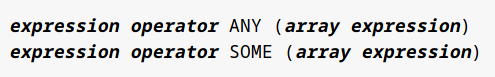
\includegraphics[width=\textwidth]{any.png}
    \caption{Gramática del operador \emph{ANY} \cite{any}}
\end{figure}

\begin{quote}\itshape
    La \textbf{expresión} del lado izquierdo es evaluada y comparada con cada elemento del \textbf{arreglo} usando el \textbf{operador} dado, el cual debe devolver un resultado lógico. El resultado de \emph{ANY} es verdader si se obtuvo por lo menos un valor verdadero. El resultado es falso si ningún valor verdadero fue devuelto \cite{any}    
\end{quote}

Dado el caso de que no se supiera el nombre exacto de la aerolínea que se quiere buscar, la consulta anterior no serviría. En tal caso, se debería hacer uso del operador \emph{ILIKE} y de las \emph{cartas bravas} (\emph{wildcards}) que provee SQL para buscar patrones \cite{pattern}.

\vspace*{5mm}
\lstset{style=sql}
\begin{lstlisting}
SELECT nombre
    FROM aeropuerto, UNNEST(aerolineas) AS nombres_aerolineas 
    WHERE nombres_aerolineas ILIKE '%argentina%';
\end{lstlisting}

Sin embargo la consulta anterior no cumpliría con la consigna debido a que se solicitaba explícitamente emplear el operador \emph{ANY}.

\subsection{Aeropuertos con todos los hangares alquilados}

\emph{Mostrar todos los aeropuertos de los cuales se tiene alquilados hangares y que estén ocupados todas las parcelas (uso del ALL) en la consulta deben aparecer los nros. de avion y descripción del modelo de avion que estén ocupando cada parcela.} 

~\\

La sintaxis del operador \emph{ALL} es idéntica a la del \emph{ANY}; evaluará a verdadero siempre y cuando la expresión indicada se cumpla para \emph{todos} los elementos del arreglo pasado a la función.   

\clearpage

\vspace*{5mm}
\lstset{style=sql}
\begin{lstlisting}
SELECT  nombre, 
        oid_avion, 
        descripcion 
FROM    aeropuerto_hangares, 
        UNNEST(espacios), 
        avion, 
        "modeloAvion" 
WHERE true = ALL(SELECT esta_ocupado FROM UNNEST(espacios)) 
    AND oid_avion=avion.oid 
    AND avion."tipoModelo"="modeloAvion"."tipoModelo" 
ORDER BY aeropuerto_hangares.ctid;
\end{lstlisting}

Debido a que la tabla \emph{aeropuerto} no tiene ninguna clave primaria, se utilizó el campo \emph{ctid} \footnote{Ubicación física de la fila en la tabla. El \emph{ctid} de una fila cambia cada vez que la fila es actualizada o movida por la operación \emph{VACUUM FULL} \cite{ctid}} (manejado internamente por el motor) para ordenar el resultado de la consulta. 


\section{Relaciones anidadas}
\emph{\textbf{El script de las consultas es \dq{consultas\_anidadas.sql}}} 

~\\

Silberschatz define el \textbf{modelo relacional anidado} como
\begin{quote}\itshape
    (El modelo relacional anidado) es una extensión del modelo relacional en la que los dominios pueden ser atómicos o de relación. Por lo tanto, el valor de las tuplas de los atributos puede ser una relación, y las relaciones pueden guardarse en otras relaciones. \cite{silberschatz}
\end{quote}

Esta extensión al sistema relacional permite crear un modelo tabular que sea más natural y cercano a la realidad, permitiendo tener tipos estructurados en una tupla o colecciones.

No obstante, las relaciones anidadas se pueden expresar en \textbf{Primera Forma Normal}, convirtiendo sus atributos complejos en atributos de dominios simples. Los tipos estructurados sencillamente se pueden pasar a \textbf{1FN} desmembrándolos en la consulta y mostrar cada uno de sus campos. Para el caso de las colecciones, se utiliza el \textbf{desanidamiento}, que transforma un arreglo en una serie de filas.

Por otra parte, también se puede expresar una relación en \textbf{1FN} como una relación anidada, utilizando el \textbf{anidamiento} (extensión de la agrupación en SQL \cite{silberschatz}); transorma un conjunto de filas (agrupadas por un criterio, con la claúsula \emph{GROUP BY}) en un arreglo.

\subsection{Normalización}
\emph{Escribir una consulta y documentar el resultado para mostrar en una tabla en 1ra Forma Normal el contenido de la tabla aeropuertosHangares. Verificar que las columnas tengan nombre significativo.} 

~\\

En \emph{Postgres}, el desanidamiento de una relación anidada se realiza con la función \textbf{unnest}. La consulta requerida se expresaría de la siguiente manera  

\vspace*{5mm}
\lstset{style=sql}
\begin{lstlisting}
SELECT  nombre AS "Aeropuerto", 
        (parcelas).numero_parcela AS "Numero de parcela", 
        CASE WHEN (parcelas).esta_ocupado=true THEN 
            'Ocupado' 
        ELSE 'Disponible' 
        END AS "Esta ocupado?", 
        (parcelas).oid_avion AS "Avion" 
FROM aeropuerto_hangares, UNNEST(espacios) AS parcelas;
\end{lstlisting}

\subsection{Desnormalización de relaciones en forma normal}
\emph{Escribir una consulta para mostrar los nombres de los trabajadores y un arreglo de todos los aviones que repararon mostrando nro de avion y descripcion del modelo, basandose en un JOIN entre las tablas avion, modeloAvion y trabajador.} 

~\\

El motor utilizado no implementa la función \textbf{nest} como tal, pero si provee de función que cumple con el mismo fin, \textbf{ARRAY\_AGG}. 

\clearpage   

\vspace*{5mm}
\lstset{style=sql}
\begin{lstlisting}
SELECT  trim(nombre) AS "Trabajador", 
        ARRAY_AGG(ROW(tr."nroAvion", trim(descripcion)))  AS "Aviones reparadas"
FROM "trabajadorReparacion" AS tr 
    JOIN trabajador AS t ON tr."dniTrabajador"=t.dni 
    JOIN avion AS av ON tr."nroAvion"=av."nroAvion" 
    JOIN "modeloAvion" AS ma ON av."tipoModelo"=ma."tipoModelo" 
GROUP BY nombre ORDER BY nombre;
\end{lstlisting}



\section{Comparación entre \emph{OODB} y \emph{RDB} extendidos}

La principal diferencia entre los dos sistemas de bases de datos se presenta justamente en el nombre; los \emph{OODB} manejan los registros  como \emph{objetos}, agregando también la gran mayoría de las características del paradigma orientado a objetos (herencia, comportamiento de los objetos, interfaces). Nótese que con \emph{registros} se hace referencia a las \dq{tuplas} de la tabla, ya que estos sistemas también implementan \textbf{valores} para representar a los tipos de datos básicos (como enteros, cadenas, o valores booleanos) para no generar una cantidad excesiva de \emph{OIDs} \cite{elmasri}.

Así como en el paradigma OO, los objetos en un \emph{OODB} cuentan con
\begin{itemize}
    \item identidad (implementado mediante el \emph{OID});
    \item comportamiento (a través de métodos);
    \item estado (compuesto por el conjunto de valores de sus atributos y vínculos con otros objetos);
    \item contructor
\end{itemize}

Cabe agregar que en \cite{silberschatz} no se habla de sistemas \emph{OODB}, sino de \emph{lenguajes de programación presistentes}, definiéndolos como \emph{lenguajes de programación extendidos con constructores para el tratamiento de datos persistentes}.

~\\

Por otro lado, los sistemas \emph{RDB} extendidos son sistemas de bases de datos relacionales con características de los sistemas \emph{OODB} agregadas. Si bien estas incorporaciones facilitan el modelado de ciertas estructuras de datos (logrando un modelo más natural), eventualmente \dq{desnormalizan} las relaciones.

Algunas de las características que añaden son:

\begin{itemize}
    \item Tipos complejos
        \begin{itemize}
            \item tipos colección;
            \item tipos estructurados
        \end{itemize}
    \item Identificadores de objetos \emph{OIDs} 
    \item Herencia
        \begin{itemize}
            \item de tipos;
            \item de tablas
        \end{itemize}
    \item Tipos \emph{referencia} 
\end{itemize}






%%%%%%%%%%%%%%%%%%%%%%%%%%%%%%%%%%%%%%%%%%%%
% FIN DOCUMENTO, AHORA REFERENCIAS
%%%%%%%%%%%%%%%%%%%%%%%%%%%%%%%%%%%%%%%%%%%%
\clearpage
\bibliographystyle{plainnat}
\bibliography{references}

\end{document}
\todo[inline, color=green!40]{This is an inline comment.}
